\chapter{The Glorious Throne and the Lamb (4:1--5:14)}\index{glory}\index{throne of God}\index{Lamb, the}

John was caught up into heaven, where he saw God seated upon the throne\index{throne of God}—the Lord of all creation, worthy of all glory\index{glory}, honor, and worship\index{worship}.
How shall we join the hosts of heaven and all creation on earth in worshiping the One who reigns forever?

\section{The Heavenly Throne and the Worship of the Four Living Creatures}\index{four living creatures}\index{worship}\index{throne of God}

% Insert the licensed NIV text of Revelation 4:1--9 in the ScriptureBox below.

\begin{ScriptureBox}

\item[4:1] After this I looked, and there before me was a door standing open in heaven. And the voice I had first heard speaking to me like a trumpet said, ``Come up here, and I will show you what must take place after this.''

\item[4:2] At once I was in the Spirit, and there before me was a throne in heaven with someone sitting on it.

\item[4:3] And the one who sat there had the appearance of jasper and ruby. A rainbow that shone like an emerald encircled the throne.

\item[4:4] Surrounding the throne were twenty-four other thrones, and seated on them were twenty-four elders. They were dressed in white and had crowns of gold on their heads.

\item[4:5] From the throne came flashes of lightning, rumblings and peals of thunder. In front of the throne, seven lamps were blazing. These are the seven spirits of God.

\item[4:6] Also in front of the throne there was what looked like a sea of glass, clear as crystal. In the center, around the throne, were four living creatures, and they were covered with eyes, in front and in back.

\item[4:7] The first living creature was like a lion, the second was like an ox, the third had a face like a man, the fourth was like a flying eagle.

\item[4:8] Each of the four living creatures had six wings and was covered with eyes all around, even under its wings. Day and night they never stop saying:\\
\hspace*{1.5em}``\,`Holy, holy, holy\\
\hspace*{1.5em}is the Lord God Almighty,'\\
\hspace*{1.5em}who was, and is, and is to come.''

\item[4:9] Whenever the living creatures give glory, honor and thanks to him who sits on the throne and who lives for ever and ever,

\end{ScriptureBox}


The heavenly throne John beheld bears a striking resemblance to the visions described by Ezekiel\index{Ezekiel} and Isaiah. As we noted in Chapter 1, both prophets were granted a glimpse of Christ's glory in times of great distress. Against the backdrop of national crisis and the rebellion of God's people, the Lord revealed a truth that no earthly turmoil could overturn: He remains sovereign over history, clothed in glory and holiness, reigning with supreme authority.

How privileged we are to receive the vision given to John! In Revelation, we are permitted to see an even fuller and more detailed portrayal of the heavenly throne than those recorded by Ezekiel and Isaiah.

Table \ref{table:rev3_comp} compares the three visions.

{
\renewcommand{\arraystretch}{1}
\small
\begin{longtable}{L{3.2cm}|L{3.2cm}|L{3.6cm}}
\caption{The throne visions of Ezekiel, Isaiah, and Revelation compared}
\label{table:rev3_comp} \\
\hline
\textbf{Ezekiel} & \textbf{Isaiah} & \textbf{Revelation} \\
\hline
1:1 The heavens were opened &
6:1 The Lord seated on a throne &
4:1 A door standing open in heaven \\
\hline
1:26 Something resembling a throne &
6:1 The Lord seated on a high and exalted throne &
4:2--3 A throne set in heaven \\
\hline
1:28 The appearance of a rainbow &
6:1--3 The glory of the Lord &
4:3 Jasper, ruby, and a rainbow around the throne \\
\hline
1:5--14 Four living creatures, later identified as cherubim\footnote{``These were the living creatures I had seen beneath the God of Israel by the Kebar River, and I realized that they were cherubim'' (Ezekiel 10:20, NIV).} &
6:2 Seraphim, each with six wings &
4:6--8 Four living creatures with six wings and eyes all around \\
\hline
1:24--28 The vision accompanied by a sound and the manifestation of glory &
6:3 ``Holy, holy, holy'' &
4:8 The four living creatures proclaim God's holiness day and night \\
\hline
1:28 Falling facedown &
6:5 ``Woe to me!'' &
1:17 John falls at Christ's feet as though dead \\
\hline
\end{longtable}
}


\begin{figure}[htbp]
    \centering
    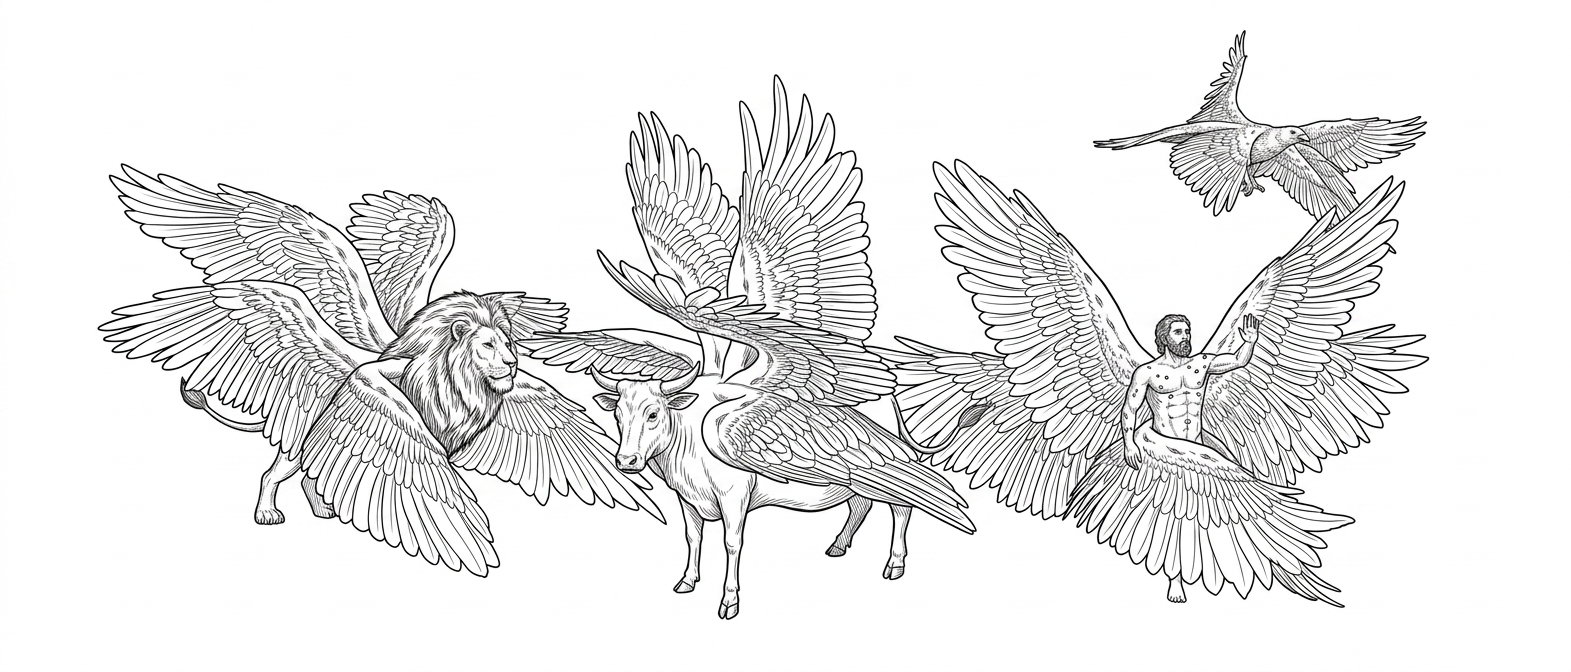
\includegraphics[
    width=1\textwidth,
    trim=100 50 100 30,
    clip]{images/four_living_creatures.jpg}
\end{figure}

The four living creatures\index{four living creatures} are beings of extraordinary power, unlike anything found among the creatures of the earth. Their bodies are covered with eyes, before and behind, within and without. They watch over all that God has made, evoking the divine knowledge that sees all things and nothing escapes His sight.\footnote{MacArthur, J. (2007); Osborne, G. R. (2002).}

Revelation 4:7 also closely parallels Ezekiel 1:10, as shown in Table \ref{table:four_creatures}:

{
\renewcommand{\arraystretch}{1}
\small
\begin{longtable}{L{4cm}L{4.5cm}}
\caption{The four living creatures in Revelation and Ezekiel}
\label{table:four_creatures} \\
\hline
\textbf{Revelation 4:7} & \textbf{Ezekiel 1:10} \\
\hline
Like a lion & The face of a lion \\
Like an ox & The face of an ox \\
Like a human being & The face of a human being \\
Like a flying eagle & The face of an eagle \\
\hline
\end{longtable}
}

\section{Praise to the Lord Who Created All Things}

% Insert the licensed NIV text of Revelation 4:10--11 in the ScriptureBox below.

\begin{ScriptureBox}

\item[4:10] the twenty-four elders fall down before him who sits on the throne and worship him who lives for ever and ever. They lay their crowns before the throne and say:

\item[4:11] \hspace*{1.5em}``You are worthy, our Lord and God,\\
\hspace*{1.5em}to receive glory and honor and power,\\
\hspace*{1.5em}for you created all things,\\
\hspace*{1.5em}and by your will they were created\\
\hspace*{1.5em}and have their being.''

\end{ScriptureBox}

The Old Testament, especially the Psalms, is filled with songs of praise to God as Creator\index{Creator}. When we read Revelation, we gain a richer understanding by setting its words alongside the related passages of Scripture. The theme of creation in Revelation 4:11 calls to mind Genesis 1, Psalm 33, Psalm 95, and Psalm 96.\footnote{Bauckham, R. (1993).}

Genesis 1 declares that in the beginning God created the heavens and the earth, and that He made humankind.

Psalm 33 proclaims the power of God's word: He speaks, and it comes to be; He commands, and it stands firm.

Psalm 95:3--7 praises the LORD as the great King above all gods. The depths of the sea, the heights of the mountains, and the whole earth belong to Him, for He made them all. Therefore, His people are called to bow down and worship Him.

Psalm 96:4--5 declares the LORD to be exalted above the gods of the nations. He made the heavens and is worthy of the worship of all peoples.

God is not merely the Creator\index{Creator} of all things; He is also the King over all creation. When the twenty-four elders\index{twenty-four elders} lay their crowns before the throne, they acknowledge that every honor and every authority possessed by created beings originates with God and must ultimately be returned to Him.

\section{No One Was Worthy to Open the Scroll}\index{scroll}

% Insert the licensed NIV text of Revelation 5:1--4 in the ScriptureBox below.

\begin{ScriptureBox}

\item[5:1] Then I saw in the right hand of him who sat on the throne a scroll with writing on both sides and sealed with seven seals.

\item[5:2] And I saw a mighty angel proclaiming in a loud voice, ``Who is worthy to break the seals and open the scroll?''

\item[5:3] But no one in heaven or on earth or under the earth could open the scroll or even look inside it.

\item[5:4] I wept and wept because no one was found who was worthy to open the scroll or look inside.

\end{ScriptureBox}

\begin{figure}[htbp]
    \centering
    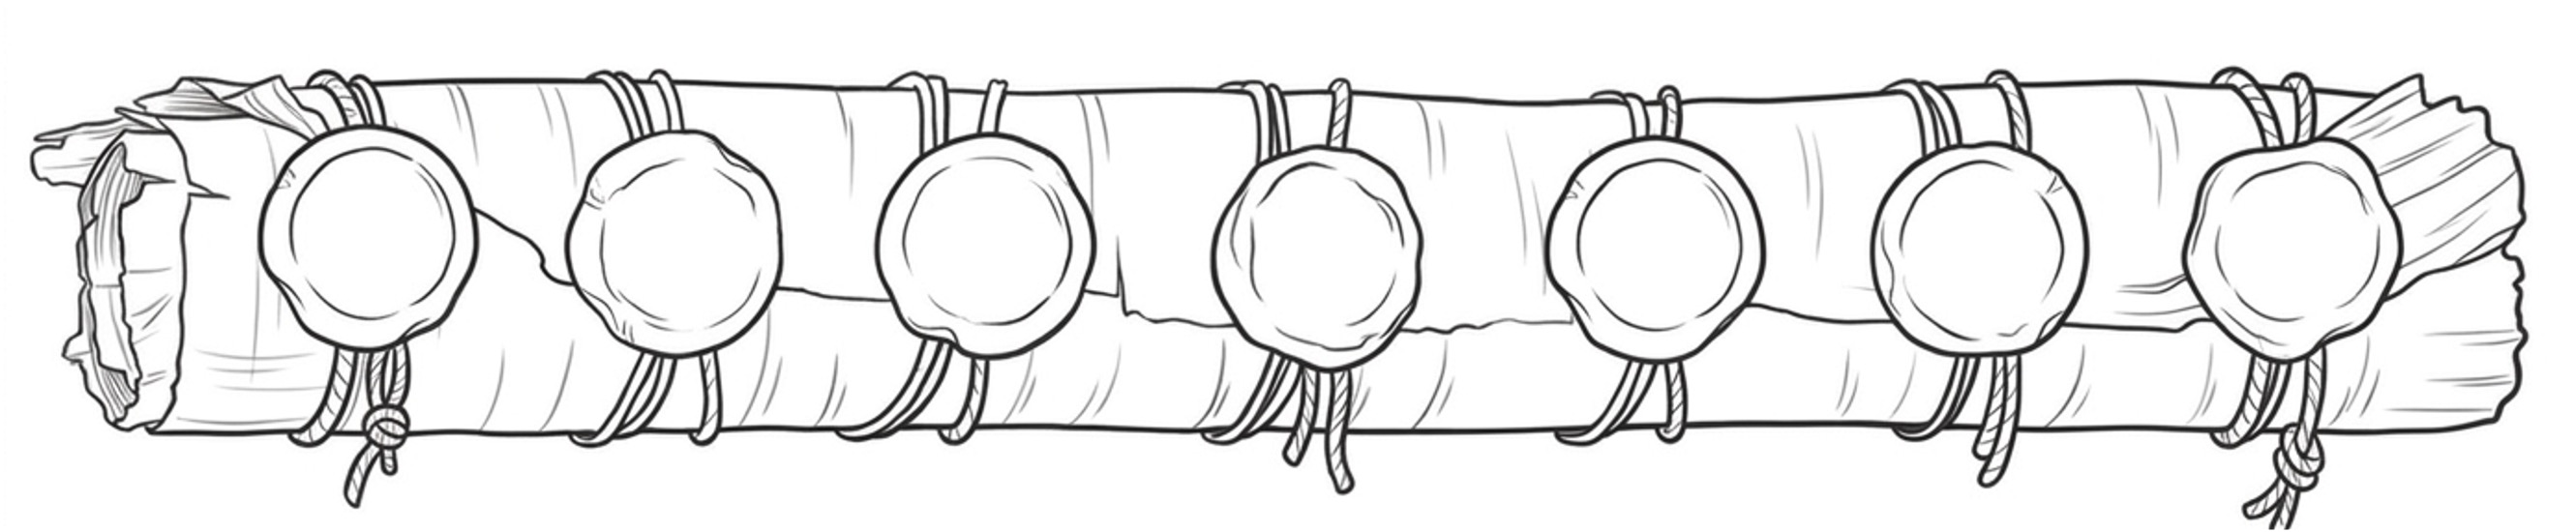
\includegraphics[
    width=1\textwidth,
    trim=0 0 0 0,
    clip]{images/scroll_light.jpg}
\end{figure}

History rests in God's hands, and the scroll\index{scroll} in His right hand holds the unfolding of His sovereign purpose. Yet who is worthy to open it, breaking its seals and bringing God's purposes to their appointed fulfillment? Not one being in all creation is found worthy. At this discovery, John weeps bitterly.

His sorrow is not merely the frustration of being unable to see what the scroll contains. The deeper anguish is that if no one is worthy to open it, no created being can bring God's plan of redemption\index{redemption} and judgment\index{judgment} into its appointed course.\footnote{This scene recalls the scroll in Ezekiel 2:9--10, which was also written on both sides. There is, however, an important difference: Ezekiel's scroll was already opened, whereas the scroll in Revelation remains sealed. Ezekiel writes, ``I looked, and I saw a hand stretched out to me. In it was a scroll, which he unrolled before me. On both sides of it were written words of lament and mourning and woe'' (Ezekiel 2:9--10, NIV).}

Why does John see an ancient scroll? If the reader lived in the modern world—or even in a distant future—would the revelation not take another form? Of course, John is not attempting to predict the technology through which future generations might publish information. He is using a means of revelation familiar to the world in which he lived.

In the ancient world, documents were commonly written on papyrus or other materials and rolled into scrolls. What John sees, therefore, is neither a modern bound book nor a digital document. The vision speaks through an image his first readers could recognize, while directing their eyes toward a purpose far greater than the scroll itself.

\section{The Slain Lamb Is the True Victorious King}\index{Lamb, the!slain}

% Insert the licensed NIV text of Revelation 5:5--7 in the ScriptureBox below.

\begin{ScriptureBox}

\item[5:5] Then one of the elders said to me, ``Do not weep! See, the Lion of the tribe of Judah, the Root of David, has triumphed. He is able to open the scroll and its seven seals.''

\item[5:6] Then I saw a Lamb, looking as if it had been slain, standing at the center of the throne, encircled by the four living creatures and the elders. The Lamb had seven horns and seven eyes, which are the seven spirits of God sent out into all the earth.

\item[5:7] He went and took the scroll from the right hand of him who sat on the throne.

\end{ScriptureBox}

Here we encounter once more the image of Jesus introduced in Chapter 1: He is the Lord who suffered and was slain, yet He is also the Lord who rose from the dead, clothed in glory and invested with authority.

The Lamb\index{Lamb, the} calls to mind His death, sacrifice, and redeeming work. The Lion of the tribe of Judah\index{Lion of the tribe of Judah} evokes His kingship, authority, and victory. Yet the Lion appears as a Lamb who has been slain. This is the wonder at the heart of Revelation: Christ accomplished redemption through His death and resurrection, and through that very victory He revealed the authority of the true King.

John then sees the Lamb with ``seven horns and seven eyes.'' The seven eyes are identified with the seven spirits\index{seven spirits} of God sent out into all the earth. In the Old Testament, a horn often symbolizes strength, power, and royal authority. The image therefore points to Christ's sovereign power and to the work of God's Spirit throughout the world.

The victorious King does not conquer\index{overcomers} as earthly rulers do. His triumph is revealed in the marks of sacrifice. The One who was slain is the One who alone is worthy to take the scroll\index{scroll} from the hand of the One seated on the throne.

\section{The Lamb Redeems People with His Own Blood}\index{redemption}\index{Lamb, the}

\begin{ScriptureBox}

\item[5:8] And when he had taken it, the four living creatures and the twenty-four elders fell down before the Lamb. Each one had a harp and they were holding golden bowls full of incense, which are the prayers of God's people.

\item[5:9] And they sang a new song, saying:\\
\hspace*{1.5em}``You are worthy to take the scroll\\
\hspace*{1.5em}and to open its seals,\\
\hspace*{1.5em}because you were slain,\\
\hspace*{1.5em}and with your blood you purchased for God\\
\hspace*{1.5em}persons from every tribe and language and people and nation.

\item[5:10] \hspace*{1.5em}You have made them to be a kingdom and priests to serve our God,\\
\hspace*{1.5em}and they will reign on the earth.''

\end{ScriptureBox}

Through His own blood, the Lamb has redeemed people from every nation and brought them to God.

This is the song of sinners who have been overtaken by grace\index{grace}. Their voices bear witness to the astonishing mercy of God, to lives transformed by His saving work, and ultimately to the glory into which He brings His redeemed people.

Christ does more than forgive our sins. He grants us a new identity, making us a kingdom and priests who belong to God. Those who were once far from Him are brought near. Those who once had no claim to stand among the worshipers of heaven are now welcomed to join their song of praise to the Lamb.

Grace has changed their standing before God, and it has changed the direction of their lives. They belong to the One who purchased them with His blood. Their redemption is not the end of their story, but the beginning of a life devoted to the worship and service of their Redeemer.

\section{From John's Weeping to the Worship of the Whole Universe}\index{worship}

\begin{ScriptureBox}

\item[5:11] Then I looked and heard the voice of many angels, numbering thousands upon thousands, and ten thousand times ten thousand. They encircled the throne and the living creatures and the elders.

\item[5:12] In a loud voice they were saying:\\
\hspace*{1.5em}``Worthy is the Lamb, who was slain,\\
\hspace*{1.5em}to receive power and wealth and wisdom and strength\\
\hspace*{1.5em}and honor and glory and praise!''

\item[5:13] Then I heard every creature in heaven and on earth and under the earth and on the sea, and all that is in them, saying:\\
\hspace*{1.5em}``To him who sits on the throne and to the Lamb\\
\hspace*{1.5em}be praise and honor and glory and power,\\
\hspace*{1.5em}for ever and ever!''

\item[5:14] The four living creatures said, ``Amen,'' and the elders fell down and worshiped.

\end{ScriptureBox}

%\begin{figure}[htbp]
%    \centering
%    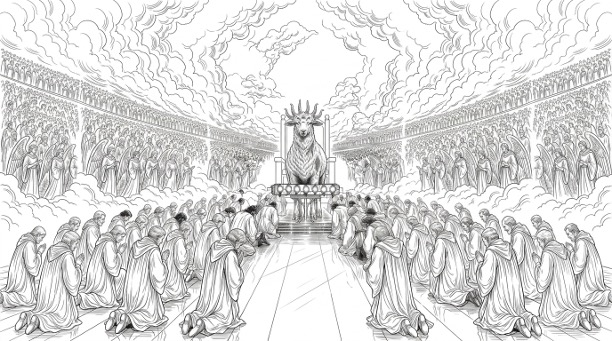
\includegraphics[
%    width=1\textwidth,
%    trim=0 0 0 0,
%    clip]{images/lamb_get_scroll2.jpg}
%\end{figure}

What a magnificent chorus of praise! The circle of worship expands from countless angels around the throne to every creature in heaven, on earth, beneath the earth, and in the sea. All creation joins in ascribing praise, honor, glory, and power to the One seated on the throne and to the Lamb, forever and ever.

Chapter 4 presents the worship due to God because He created all things. Chapter 5 reveals the worship due to the Lamb because He accomplished redemption. Creation and redemption converge in one great act of adoration: the Lamb who was slain\index{Lamb, the!slain}, and who lives forever, receives eternal worship together with the One seated on the throne.

Table \ref{table:rev4_5_praise} summarizes the relationship between these two chapters for their reason of praise, worshipers, and central message.

{
\renewcommand{\arraystretch}{1}
\small
\begin{longtable}{L{4.5cm}L{4.5cm}}
\caption{Praise for creation and praise for redemption in Revelation 4--5}
\label{table:rev4_5_praise} \\
\hline
\textbf{Chapter 4: Praise for Creation} & \textbf{Chapter 5: Praise for Redemption} \\
\hline
The Lord seated on the throne &
The Lord seated on the throne and the Lamb \\

God created all things &
The Lamb was slain and redeemed people with His blood \\

Glory, honor, power, and the creation of all things &
Power, wealth, wisdom, strength, honor, glory, and praise \\

The four living creatures and the twenty-four elders &
The four living creatures, the twenty-four elders, countless angels, and all created beings \\

All things were created according to God's will &
People from every nation are redeemed by the Lamb's blood and brought to God \\
\hline
\end{longtable}
}

Creation and redemption meet in this heavenly vision. The Lamb who was slain\index{Lamb, the!slain}, and who now lives, receives eternal worship together with God upon the throne.

May we praise Him each day for the power by which He created all things, letting our words of praise surge like the boundless sea. May we also give thanks each day for the grace by which He redeemed us, letting our gratitude flow like a mighty river, never running dry.

For we were not merely brought into existence by the Creator\index{Creator}; through the blood of the Lamb\index{Lamb, the!blood of}, we have been brought near to Him. The One who reigns over all creation has made a way for sinners to stand before His throne. Here lies the wonder of grace: those who once had no reason to boast now have every reason to worship.

\section*{Discussion Questions}

\begin{enumerate}

\item In the days when Israel faced national disaster and God's people endured suffering, Ezekiel and Isaiah were also given visions of God's glorious throne. How do these visions help us understand that God remains sovereign over history? What do they teach us when we face hardship and uncertainty in our own lives?

\item The four living creatures proclaim without ceasing, ``Holy, holy, holy is the Lord God Almighty, who was, and is, and is to come.'' What do God's holiness, eternity, and omnipotence mean for our worship today? How should these truths shape the way we approach Him?

\item Genesis 1 and Psalms 33, 95, and 96 praise God's creation from different perspectives. How should recognizing God as the Creator of all things change the way we view our lives, our work, and the created world around us?

\end{enumerate}
